\section{Le Patch}
\label{sec:adapter_patch}

Tout d'abord, il faut peut être ajuster le patch. Peut être des adresses doivent être changées ? Pas de soucis ! C'est le moment de le faire.
\newline
La seule rêgle ici : ne JAMAIS supprimer une fixture du patch, sans quoi toute son encod est définitivement perdue.
\newline
Si vous avez besoin de rajouter des projecteurs de dernière minute, changer un mode ou un type de projecteur, c'est ici que ça se passe.

\subsection{Changer un type de projecteur}
\label{subsec:fixture_morph}

L'opération que nous allons faire ici est appelée "Morphing". Cela consiste à changer le type de projecteur d'une fixture sans perdre la programmation déjà faite.
\newline
Sur le principe, la Chimp fonctionne par "attributs". C'est à dire que chaque fixture a un certain nombre d'attributs (couleur, position, gobo, etc.) et que ces attributs sont controlés par des canaux DMX.
Changer un typ ou mode de projecteur pour un autre ne change pas fondamentalement les attributs (si elles sont similaires), mais change juste la manière dont ces attributs sont associés au canaux DMX.
Pour en savoir plus, voir la section \ref{subsec:fixture_patch}.
\newline
On peut donc selectionner une ou plusieurs fixtures dans le patch, et appuyer sur \textit{Change Type} pour changer le type de projecteur.
Il faut être vigilant cependant à ce qu'il n'y ai pas de débordement dans les adresses DMX. Si le nouveau type de projecteur a plus de canaux DMX que l'ancien, cela devra avoir été anticipé dans le patch (en prévoyant un décalage dans les adresses DMX),
ou alors il faudra réadresser une partie de cet univers.
\newline
\newline
Si votre problème est que le projecteur n'est pas disponible dans la librairie de votre visualisateur, il faut choisir un projecteur qui soit le plus ressemblant possible. Une fois les presets et une partie des executeurs faits \textbf{sur la bonne fixture}, vous pouvez alors faire un morphing pour changer le type de projecteur.
Vous reviendrez alors sur la fixture d'origine quand vous aurez le bon projecteur dans la librairie de votre visualisateur, ou que vous êtes devant le projecteur en vrai.
\newline
\newline
\textbf{Attention :} Si vous changez le type de projecteur, il est possible que les presets de couleurs, positions, gobos, etc. ne soient plus adaptés. Il faudra donc les revoir (voir section \ref{sec:adapter_presets}).
\newline
\textbf{Attention 2 :} Parfois, le morphing peut échouer. C'est particulièrement le cas pour des fixtures qui possèdent plusieurs instances. Dans ce cas$\dots$ il n'y a pas de solution miracle. Il faudra réencoder la fixture.

\subsection{Cloner une fixture}
\label{subsec:cloner_fixture}

Parfois, on peut décider au dernier moment de rajouter un projecteur sur le plan de feu. Problème : il n'a aucune encod.
\newline
Pas de soucis ! Il suffit de cloner une fixture déjà existante.
\newline
Dans un premier temps, patchez et identifiez le nouveau projecteur. Ensuite, ouvrez le menu \textit{Clone Fixture} dans le patch, et selectionnez la source et la destination.
La fenêtre doit ressembler à ça :
\begin{figure}[H]
    \centering
    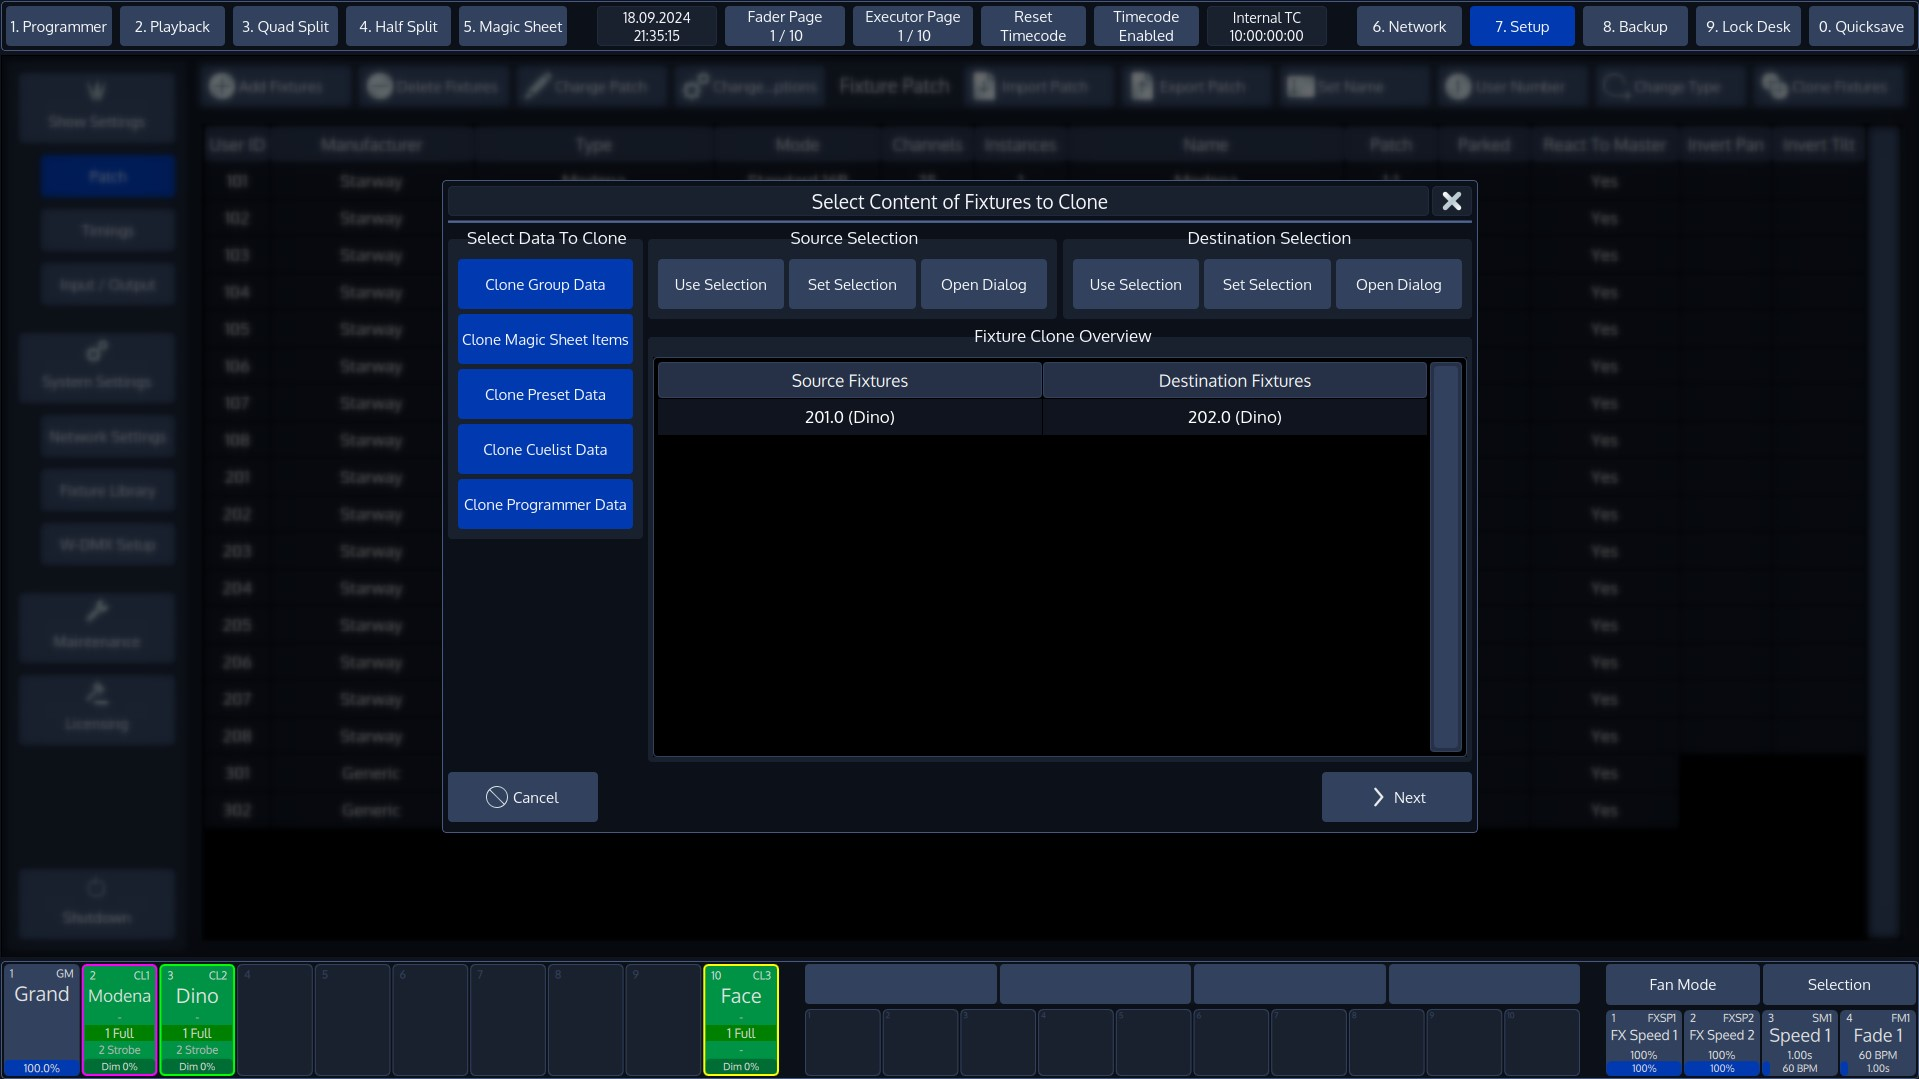
\includegraphics[width=\textwidth]{4 - Adapter la programmation/Images/clone_fixture.jpg}
    \caption{Fenêtre de clonage de fixture}
\end{figure}
Les données de programmation sont alors copiées de la fixture source à la fixture destination. Il ne reste plus qu'à adapter les presets.

\subsection{Pan/Tilt Invert}
\label{subsec:invert_pan_tilt}

De la même manière que cela a été fait lors du patch sur la console, il faut verifier que toutes les fixtures se déplacent toutes dans le même sens.
\newline
Voir section \ref{subsec:prep_invert} pour plus d'informations.
